
\documentclass[a4paper,12pt]{article}
\usepackage[ngerman]{babel}
% \usepackage[ngerman]{babel}
\usepackage[utf8]{inputenc}
\usepackage[T1]{fontenc}
\usepackage{lmodern}
\usepackage{titling}
\usepackage{geometry}
\geometry{left=3cm, right=3cm, top=2cm, bottom=3cm}
\usepackage{setspace}
\onehalfspacing

\usepackage{ifthen}

\usepackage{graphicx}
% \usepackage{pstricks}
% \usepackage{relsize}
% \usepackage[decimalsymbol=comma,exponent-product = \cdot, per=frac]{siunitx}
% \sisetup{range-phrase=\,bis\,}

\usepackage{xargs}
\usepackage{calc}
\usepackage{amsmath}
\usepackage{amsfonts}
\usepackage{mathtools}
\usepackage{amssymb}

\usepackage{cancel}
\usepackage{trfsigns}
\usepackage{array}
\usepackage{enumerate}
\usepackage{enumitem}

\usepackage{caption}
\usepackage{subcaption}

\usepackage{multicol}

\usepackage{pdflscape}
\usepackage[table]{xcolor}

\usepackage{float}

%%%%%%%%%%%%%%%%%%%%%%%%%%%%%%%%%%%%%%%%%%%%%%%%%%%%%%%%%%%%%%%%%%%%%%%%%%%%%%%%
\newboolean{WITHPSTRICKS}
\setboolean{WITHPSTRICKS}{false}


\newcommand{\PROFESSOR}{Prof.\ Dr.\ Thomas Carraro}
\newcommand{\ASSISTANT}{\setlength{\tabcolsep}{0pt}\begin{tabular}{l}\end{tabular}}

\newcommand{\Jahr}{2022}
% \newcommand{\Trimester}{HT}
\newcommand{\Trimester}{WT-FT}
\newcommand{\Kurs}{Mathematik II-III}
\newcommand{\TYPE}{Aufgabenblatt}
\newcommand{\BLATT}{1}
\newcommand{\TOPIC}{}

%%%%%%%%%%%%%%%%%%%%%%%%%%%%%%%%%%%%%%%%%%%%%%%%%%%%%%%%%%%%%%%%%%%%%%%%%%%%%%%%
\newboolean{mitLoes}
\setboolean{mitLoes}{false}
 \setboolean{mitLoes}{true}

%%%%%%%%%%%%%%%%%%%%%%%%%%%%%%%%%%%%%%%%%%%%%%%%%%%%%%%%%%%%%%%%%%%%%%%%%%%%%%%%


%\setboolean{WITHPSTRICKS}{false}
%\setboolean{WITHPSTRICKS}{true}


\usepackage{tikz}
\usetikzlibrary{arrows,automata,backgrounds,calendar,decorations.pathmorphing,fadings,shadings,calc,intersections}
\usetikzlibrary{decorations.pathreplacing}
\usetikzlibrary{decorations.shapes}
\usetikzlibrary{decorations.footprints}
\usetikzlibrary{decorations.text}
\usetikzlibrary{positioning}
\usetikzlibrary{through}

\ifthenelse{\boolean{WITHPSTRICKS}}{%
\usepackage{auto-pst-pdf}
\usepackage{pstricks,pst-plot,pst-text}
}{}

\usepackage{pgfplots}

%%%%%%%%%%%%%%%%%%%%%%%%%%%%%%%%%%%%%%%%%%%%%%%%%%%%%%%%%%%%%%%%%%%%%%%%%%%%%%%%
\usepackage{mbdefAufgaben}

%%%%%%%%%%%%%%%%%%%%%%%%%%%%%%%%%%%%%%%%%%%%%%%%%%%%%%%%%%%%%%%%%%%%%%%%%%%%%%%%
\newboolean{mitErg}
\setboolean{mitErg}{false}

%%%%%%%%%%%%%%%%%%%%%%%%%%%%%%%%%%%%%%%%%%%%%%%%%%%%%%%%%%%%%%%%%%%%%%%%%%%%%%%%
\newcounter{Aufg}
\setcounter{Aufg}{0}
\newcounter{Blatt}
\setcounter{Blatt}{\BLATT}

%%%%%%%%%%%%%%%%%%%%%%%%%%%%%%%%%%%%%%%%%%%%%%%%%%%%%%%%%%%%%%%%%%%%%%%%%%%%%%%%
\usepackage{KopfKlausur}

% Seitenraender
\textwidth = 285mm
\textheight = 180mm
\leftmargin 5mm
\oddsidemargin = -20mm
\evensidemargin = -20mm
\topmargin = -25mm
\parindent 0cm
\columnsep 2cm

% % % Aufgabenstellung
% % % Schwierungkeitsgrad mit "e" , "f" oder "v" angeben
% % % "e" Einführung   
% % % "f" Festigung
% % % "v" Vertiefung  

\newcommand{\Aufgabe}[3][]{
\stepcounter{Aufg}
\subsubsection*{Aufgabe 
\arabic{Blatt}.\arabic{Aufg}\ifthenelse{\equal{#1}{e}}{}{\ifthenelse{\equal{#1}{f}}{
$\!\!{}^\star$}{\ifthenelse{\equal{#1}{v}}{$^{\star\star}$}{}}}{: #2}}
{#3}
}
% % % Ergebnisse jeweils am Ende des Aufgabenblattes Anzeigen
\newcommand{\Ergebnisse}{}
\makeatletter
\newcommand{\Ergebnis}[1]{
	\g@addto@macro{\Ergebnisse}{#1}
}
\makeatother
\makeatletter
\newcommand{\ErgebnisC}[2]{
\@ifundefined{c@#1}
{\newcounter{#1}}
{}
\setcounter{#1}{\theAufg}

\ifthenelse{\boolean{mitErg}}{	\g@addto@macro{\Ergebnisse}{\subsubsection*{Ergebnisse zu Aufgabe \arabic{Blatt}.\arabic{#1}:}
}%
	\g@addto@macro{\Ergebnisse}{#2}}{}
}
\makeatother


% % % Lösungen
\newcommand{\Loesung}[1]{
	\ifthenelse{\boolean{mitLoes}}
	{\subsubsection*{Lösung \arabic{Blatt}.\arabic{Aufg}:}
		#1}
	{}
}
% % % % % % % % % % % % % % % % % % % % % % % % % % % % % % % % % % % % % % % % % % % % % % % % % % % % % %
% % % % % % % % % % % % % % % % % % % % % % % % % % % % % % % % % % % % % % % % % % % % % % % % % % % % % %
% % % % % % % % % % % % % % % % % % % % % % % % % % % % % % % % % % % % % % % % % % % % % % % % % % % % % %
\begin{document}
\begin{twocolumn}
% % % % % % % % % % % % % % % % % % % % % % % % % % %

%%%%%%%%%%%%%%%%%%%%%%%%%%%%%%%%%%%%%%%%%%%%%%%%%%%%%%%%%%%%%%%%%%%%%%%%%%%%%%%%
% Set the TITLE of the sheet here:
%\uebheader{\Kurs}{\arabic{Blatt}}{\Trimester\,\Jahr}{\TOPIC}
%\uebheader{\Kurs}{\arabic{Blatt}}{\Trimester\,\Jahr}{\TOPIC}
\uebheader{\Kurs}{\arabic{Blatt}}{\Trimester\,\Jahr}{\TOPIC}
\ruleBig

\setboolean{mitErg}{false}
% \setboolean{mitErg}{true}


%%%%%%%%%%%%%%%%%%%%%%%%%%%%%%%%%%%%%%%%%%%%%%%%%%%%%%%%%%%%%%%%%%%%%%%%%%%%%%%%
% Set the INTRODUCTION section of the sheet here:
% \input{introduction.tex}

%\textbf{Einführende Bemerkungen}

%\begin{itemize}
%\item Vermeiden Sie die Verwendung von Taschenrechnern oder Online-Ressourcen.
%\item Die mit einem Stern *) markierten (Teil-)Aufgaben entfallen in diesem Trimester. Stattdessen werden einzelne Online-Aufgaben im ILIAS-Kurs kenntlich gemacht, zu denen Sie dort Ihre L\"osungswege zur Korrektur hochladen k\"onnen. 
%\item Die mit zwei Sternen  **) markierten (Teil-)Aufgaben richten sich an Studierende, die die \"ubrigen Aufgaben bereits gel\"ost haben und die Inhalte weiter vertiefen m\"ochten. 
%\end{itemize}

%\ruleBig

%Mathe II Blatt 1

\Aufgabe[e]{Stationäre Punkte}{
Gegeben sei die Funktion $$f(x,y) := \frac1y - \frac1x - 4x + y.$$ Finde alle stationären Punkte und bestimme, ob sie lokale Minima, Maxima oder Sattelpunkte sind.
}
\Loesung{
Die stationären Punkte sind die Lösungen des folgenden Gleichungssystems%
\begin{eqnarray*}
\frac{\partial}{\partial x} f(x,y) = 0 \quad&\Rightarrow& \quad \frac{1}{x^2} - 4 = 0 \\\
\frac{\partial}{\partial y} f(x,y) = 0 \quad&\Rightarrow& \quad -\frac{1}{y^2} + 1 = 0
\end{eqnarray*}
%
Die Lösungen sind $x_{1,2} = \pm \frac12$ und $y_{1,2} = \pm 1$.

Es gibt also 4 stationäre Punkte, nämlich $(\frac{1}{2}, 1), (\frac{1}{2}, -1), (-\frac{1}{2}, 1), (-\frac{1}{2}, -1)$.

Die Hessische Matrix ist:
$$
\begin{pmatrix}
f_{xx}(x,y) & f_{xy}(x,y) \\
f_{xy}(x,y) & f_{yy}(x,y)
\end{pmatrix}
=
\begin{pmatrix}
-\frac{2}{x^3} & 0 \\\
0 & \frac{2}{y^3}
\end{pmatrix}.
$$

Charakterisierung der stationären Punkte:
$$
\boldsymbol{x}_1 = \begin{pmatrix} \frac{1}{2} \\\ 1 \end{pmatrix}, \quad \begin{pmatrix} -16 & 0 \\\ 0 & 2 \end{pmatrix}, \quad \mbox{Sattelpunkt}
$$
%
$$
\boldsymbol{x}_2 = \begin{pmatrix} \frac{1}{2} \\ -1 \end{pmatrix}, \quad \begin{pmatrix} -16 & 0 \\\ 0 & -2 \end{pmatrix}, \quad \mbox{Maximum}
$$
%
$$
\boldsymbol{x}_3 = \begin{pmatrix} -\frac{1}{2} \\ 1 \end{pmatrix}, \quad \begin{pmatrix} 16 & 0 \\\ 0 & 2 \end{pmatrix}, \quad \mbox{Minimum}
$$
%
$$
\boldsymbol{x}_4 = \begin{pmatrix} -\frac{1}{2} \\ -1 \end{pmatrix}, \quad \begin{pmatrix} 16 & 0 \\\ 0 & -2 \end{pmatrix}, \quad \mbox{Sattelpunkt}
$$

\rule{360pt}{1pt}
\cleardoublepage
}

\ifthenelse{\boolean{mitLoes}}{\ruleBig \cleardoublepage}

\Aufgabe[e]{Differentialgleichungen}{
\begin{abc}
\item
Es sei das folgende Anfangswertproblem für $y(t)$ gegeben
$$
y''(t)+3y'(t)+2y(t)= 1-h(t-1),\quad\quad y(0)=0,\ y'(0)=1.
$$
Berechnen Sie die Lösung mit Hilfe der Laplace-Transformation. Drücken Sie die Lösung in den Bereichen $0\leq t< 1$ und $t\ge 1$ ohne die Heaviside-Funktion aus.
%
\item Es sei das folgende Anfangswertproblem für $u(t)$ gegeben
$$
u''(t)+4u'(t)+4u(t)= %4t+
8e^{-2t},\quad\quad u(0)=2,\ y(0)=2.
$$
Berechnen Sie die Lösung mit Hilfe des Exponentialansatzes.
\end{abc}
}

\Loesung{
\begin{abc}
        \item Mit $\mathcal{L}\{y(t)\}=Y(s)$ ist die Laplace-Transformation des AWP
        \begin{eqnarray*}
        s^2Y(s)-1+3(sY(s))+2Y(s)&=&\dfrac{1}{s}-\dfrac{e^{-s}}{s}\\
        Y(s)(s^2+3s+2)&=&\dfrac{1}{s}-\dfrac{e^{-s}}{s}+\dfrac{s}{s}\\
                                &=&\dfrac{1}{(s+1)(s+2)}\cdot\left(\dfrac{1+s-e^{-s}}{s}\right)\\
                                &=&\dfrac{1+s}{(s+1)(s+2)s}-\dfrac{e^{-s}}{(s+1)(s+2)s}\\
                                &=&\dfrac{1}{(s+2)s}-\dfrac{e^{-s}}{(s+1)(s+2)s}
        \end{eqnarray*}
        Durch Partialbruchzerlegung des ersten und zweiten Terms erhält man
        \begin{eqnarray*}
        \dfrac{1}{s(s+2)}&=&\dfrac{1}{2}\dfrac{1}{s}-\dfrac{1}{2}\dfrac{1}{s+2}\\
        \dfrac{1}{s(s+2)(s+1)}&=&\dfrac{1}{2}\dfrac{1}{s}+\dfrac{1}{2}\dfrac{1}{s+2}-\dfrac{1}{s+1}
        \end{eqnarray*}
        Daraus folgt,
        \begin{eqnarray*}
        Y(s)&=&\dfrac{1}{2}\dfrac{1}{s}-\dfrac{1}{2}\dfrac{1}{s+2}-\left(\dfrac{1}{2}\dfrac{1}{s}+\dfrac{1}{2}\dfrac{1}{s+2}-\dfrac{1}{s+1}\right)e^{-s}\\
        \mathcal{L}^{-1}\{Y(s)\}&=&\mathcal{L}^{-1}\left\{\dfrac{1}{2}\dfrac{1}{s}-\dfrac{1}{2}\dfrac{1}{s+2}\right\}- \mathcal{L}^{-1}\left\{\left(\dfrac{1}{2}\dfrac{1}{s}+\dfrac{1}{2}\dfrac{1}{s+2}-\dfrac{1}{s+1}\right)e^{-s}\right\}\\
        y(t)&=&\dfrac{1}{2}-\dfrac{1}{2}e^{-2t}-\left(\dfrac{1}{2}+\dfrac{1}{2}e^{-2(t-1)}-e^{-(t-1)}\right)h(t-1)\\
        y(t)&=&\begin{cases}
                \dfrac{1}{2}-\dfrac{1}{2}e^{-2t} & 0\leq t<1\\[10pt]
                -\dfrac{e^{-2t}}{2}(1+e^2)+e^{-(t-1)}& t\geq 1
                \end{cases}
        \end{eqnarray*}

        \item Das charakteristische Polynom ist
        $$
        \lambda^2+4\lambda+4=0\Rightarrow \lambda_{1,2}=-2.
        $$
        Die Lösung der homogenen Differentialgleichung lautet also
        $$
        u_h(t)=(c_1+c_2t)e^{-2t}
        $$
        Wir raten eine bestimmte Lösung gemäß der rechten Seite
        \begin{align*}
        8e^{-2t}&\Rightarrow u_{p}=Ct^2e^{-2t} & &\Rightarrow u_{p}=4t^2e^{-2t}
        \end{align*}
        Die allgemeine Lösung lautet
        $$
        u(t)=u_h(t)+u_{p}(t)=(c_1+c_2t+4t^2)e^{-2t}.
        $$
        Aus $u(0)=2$ folgt $ c_1=2$ und aus $u'(0)=2$ folgt $c_2=6$ also,
        $$
        u(t)=(2+6t+4t^2)e^{-2t}.
        $$

\end{abc}

}

\ifthenelse{\boolean{mitLoes}}{\ruleBig \cleardoublepage}
\newpage
\Aufgabe[e]{Integrale in $\mathbb R^3$}{
Man betrachte die Kugel
$$K := \left\{ (x,y,z)^{\top} \in \mathbb{R}^3 \mid x^2+y^2+z^2 \leq 4\right\}.$$
Das Volume des Zylinders $$Z := \left\{ (x,y,z)^{\top} \in \mathbb{R}^3 \mid x^2+y^2 \leq 1\right\}$$ wird von der Kugel abgezogen. Bestimmen Sie das Volumen des resultierenden Körpers.

\vspace{1ex}
Hinweis: Man verwendet Zylinderkoordinaten. Das Volumen einer Kugel mit dem Radius $R$ ist $\displaystyle \frac{4}{3}\pi R^3$.
\begin{figure}[h!]
\centering
\begin{tabular}{cc}
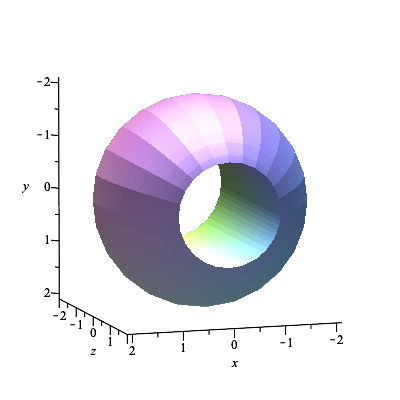
\includegraphics[width=0.5\linewidth]{../A/Wiederholung/figex3b.png}&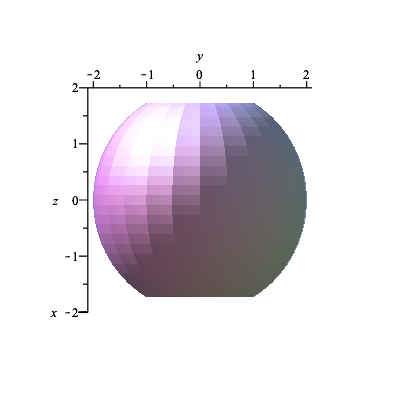
\includegraphics[width=0.5\linewidth]{../A/Wiederholung/figex3a.png}
\end{tabular}
\end{figure}
}

\Loesung{
Wir berechnen zunächst das Volumen des extrahierten Zylinders über der Ebene $(x,y)$, bezeichnet mit $G$. Dazu verwenden wir die zylindrischen Koordinaten und die entsprechenden Transformationen
$$
\begin{pmatrix}
 x\\y\\z
\end{pmatrix}
=
\begin{pmatrix}
 r \cos(\varphi)\\ r \sin(\varphi)\\ z
\end{pmatrix}.
$$
wobei $r \in [0,1],\ \varphi \in [0, 2\pi)$ und da wir nur das Volumen oberhalb der $(x,y)$-Ebene berechnen, $z\geq 0$. Die obere Grenze für $z$ wird aus der Kugelgleichung wie folgt berechnet:
\begin{eqnarray*}
x^2+y^2+z^2 &\leq &4 \\
r^2 + z ^2 &\leq &4 \\
z &\leq& \sqrt{4 - r^2} 
\end{eqnarray*}
Daraus folgt,
$$
G = \left\{
(r,\varphi,z) : 1 \leq r \leq 2,\ 0 \leq \varphi \leq 2
\pi,\ 0 \leq z \leq \sqrt{4 - r^2} \right\}.
$$
Das Volumen wird durch Integration des Volumenelements in zylindrischen Koordinaten wie folgt berechnet
\begin{eqnarray*}
\iiint\limits_{G} r \, \mathrm{d}r \, \mathrm{d}\varphi \, \mathrm{d}z &=&
 \int \limits_{0}^{2 \pi} \int \limits^{2}_{1}  \int \limits_{0}^{\sqrt{4-r^2}}
r \, \mathrm{d}z \, \mathrm{d}r \, \mathrm{d}\varphi   
= \int\limits_{0}^{2 \pi} \int\limits^{2}_{1} r \int \limits_{0}^{\sqrt{4-r^2}}
 \, \mathrm{d}z \, \mathrm{d}\varphi \, \mathrm{d}r \, \\\
&= &\int\limits_{0}^{2\pi} \int\limits_{1}^{2} r \sqrt{4 - r^2} \, \mathrm{d}r
\, \mathrm{d}\varphi \overset{t:=4-r^2}{=} \int\limits_{0}^{2\pi} -\frac12 \int\limits_{3}^{0} \sqrt{t} \, \mathrm{d}t \, \mathrm{d}\varphi \\\ 
&= & 2 \pi \sqrt{3}.
\end{eqnarray*}
Das Volumen der Kugel nach Abzug des Zylinders $Z$ ist das Integral mal zwei, weil wir nur den oberen Teil des Körpers integriert haben
$$
K \setminus Z = 4 \sqrt{3} \pi.
$$


\rule{360pt}{1pt}
\cleardoublepage
}

\ifthenelse{\boolean{mitLoes}}{\ruleBig \cleardoublepage}

\ifthenelse{\boolean{mitLoes}}{\cleardoublepage}{}
\ifthenelse{\boolean{mitErg}}{
\ruleBig
\Ergebnisse}{}


\end{twocolumn}
\end{document}
